\documentclass{article}
\usepackage[utf8]{inputenc}
\usepackage[margin = 1 in]{geometry}
\usepackage{listings}
\usepackage{xcolor}
\usepackage{booktabs}
\usepackage{graphicx}


\definecolor{codegreen}{rgb}{0, 0.6, 0}
\definecolor{codegray}{rgb}{0.5, 0.5, 0.5}
\definecolor{codepurple}{rgb}{0.58, 0, 0.82}
\definecolor{backcolour}{rgb}{0.95, 0.95, 0.92}

\lstdefinestyle{mystyle}
{
	backgroundcolor =\color{backcolour},
	commentstyle =\color{codegreen},
	keywordstyle =\color{magenta},
	numberstyle =\tiny\color{codegray},
	stringstyle =\color{codepurple},
	basicstyle =\ttfamily\footnotesize,
	breakatwhitespace = false,
	breaklines = true,
	captionpos = b,
	keepspaces = true,
	numbers = left,
	numbersep = 5pt,
	showspaces = false,
	showstringspaces = false,
	showtabs = false,
	tabsize = 2
}

\lstset{style = mystyle}
\begin{document}
\begin{titlepage} % Suppresses displaying the page number on the title page and the subsequent page counts as page 1

\raggedleft\rule{1pt}{\textheight} % Vertical line
\hspace{0.05\textwidth} % Whitespace between the vertical line and title page text
\parbox[b]{0.75\textwidth}
	{% Paragraph box for holding the title page text, adjust the width to move the title page left or right on the page

            {\Huge\bfseries MIT World Peace University \\[0.5\baselineskip] \ SET}\\[2\baselineskip] % Title
            {\large\textit{Assignment 5}}\\[4\baselineskip] % Subtitle or further description
            {\Large\textsc{Naman Soni Roll No. 10}} % Author name, lower case for consistent small caps

   \vspace{0.5\textheight} % Whitespace between the title block and the publisher
   }

\end{titlepage}
\tableofcontents
\pagebreak
\section{\textbf{Aim}}
Object Oriented Analysis and design using UML diagrams: Sequence diagram to show message exchanges, using Open Source Tool.
\section{\textbf{Objective}}
\begin{itemize}
	\item To learn the relationships and notions of Sequence Diagram.
\end{itemize}
\section{\textbf{Problem Statement}}
\textbf{Draw UML Use Case Diagram and Class Diagram for the following problem statement:} The restaurant industry is a fast-paced environment that requires efficient management of resources to ensure timely and quality service. In the traditional restaurant setting, the ordering process, food preparation, and inventory management are carried out manually, leading to errors, delays, and inefficiencies.
\section{\textbf{Theory}}
\subsection{\textit{Sequence Diagram}}
A Sequence Diagram is a type of UML (Unified Modeling Language) diagram used to visualize the interactions between objects or components in a system. It represents the flow of messages and events exchanged between different elements of a system in a sequential order.\\

A sequence diagram consists of a vertical axis representing time and horizontal arrows representing messages exchanged between objects. Each object or component involved in the interaction is represented by a vertical bar called a lifeline, which spans the entire length of the diagram. Each message or event is represented by an arrow pointing from the sender to the receiver, indicating the flow of control between them.\\

In addition to the messages exchanged between objects, sequence diagrams may also include other types of nota- tions, such as activation bars to indicate the period of time during which an object is performing an operation, and loops and conditions to represent the control flow of a system.\\

Sequence diagrams are commonly used in software engineering to model the behavior of a system and to help identify potential issues or improvements in the system design. They are particularly useful in visualizing the interactions between objects or components in complex systems.
\begin{center}
	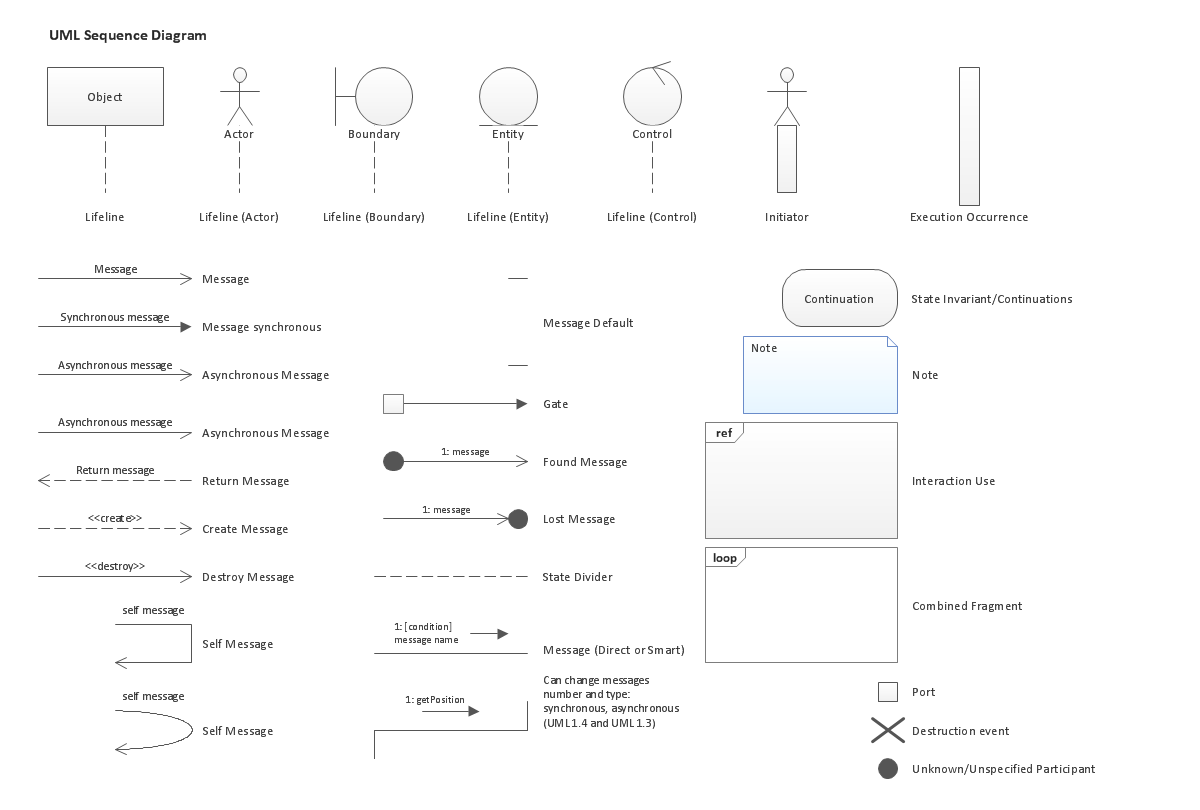
\includegraphics[scale = 0.5]{notations.png}
\end{center}
\textbf{Diffrent notations of Sequence Diagram:}
\begin{itemize}
	\item \textbf{Lifeline:} A lifeline is a vertical line that represents an object or a role in a sequence diagram. It is used to show the existence of an object or a role in a sequence diagram. It is also used to show the time duration of an object or a role in a sequence diagram.
	\item \textbf{Message:} It is an arrow that represents a communication between two objects. It can be either synchronous or asynchronous. A synchronous message is represented by a solid arrow, whereas an asynchronous message is represented by a dashed arrow.
	\item \textbf{ActivationBar:} Itisarectangularboxthatrepresentstheperiodoftimeduringwhichanobjectisexecuting a specific operation. It starts when the object receives a message and ends when the operation is completed.
	\item \textbf{Return Message:} It is a dashed arrow that represents the response sent by the receiver object to the sender object. It is used to indicate the completion of an operation.
	\item \textbf{Self Message:} It is a message that is sent by an object to itself. It is represented by a looped arrow that points back to the object.
	\item \textbf{Combined Fragment:} It is a box that represents a condition, loop, or an alternative flow of control in the system. It is represented by a rectangle with a keyword, such as ``if'', ``while,'' or ``alt,'' written inside.
	\item \textbf{Interaction Use:} It is a notation that represents a sequence diagram that is used as a sub-sequence in another diagram. It is represented by a rectangular box with a reference to the sub-sequence diagram.
\end{itemize}
\section{\textbf{Sequence Diagram}}
\begin{center}
	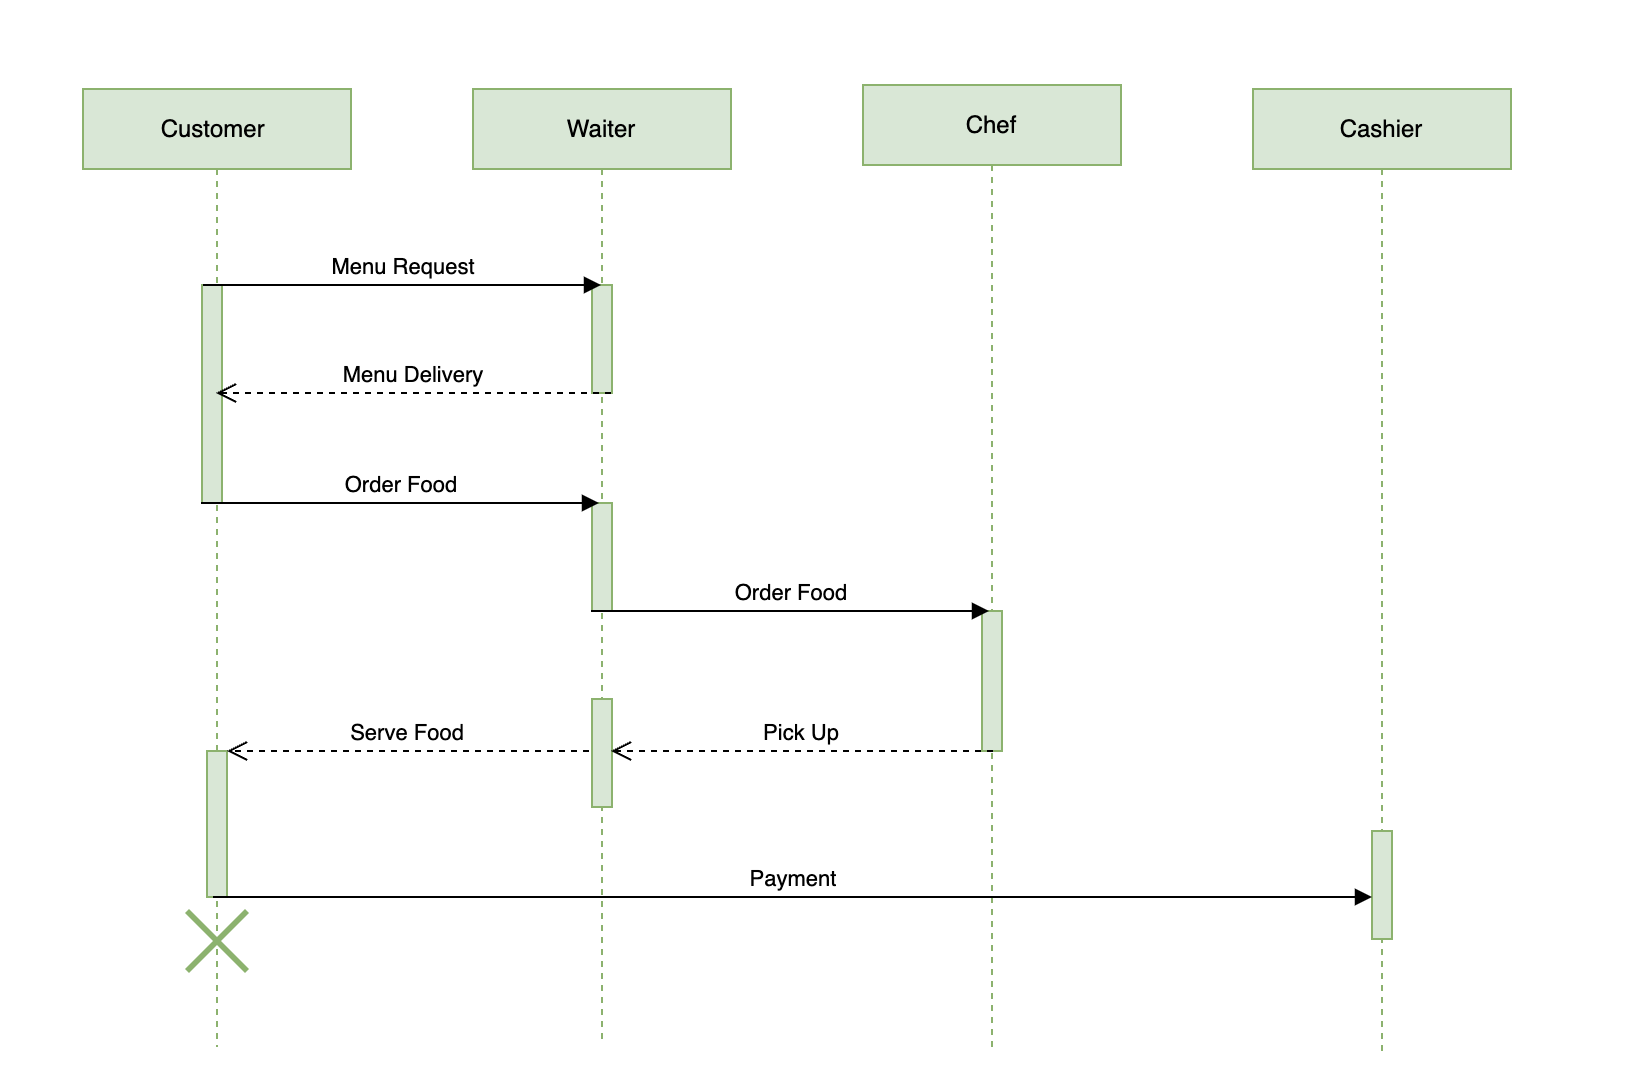
\includegraphics[scale = 0.5]{Sequence Diagram.png}
\end{center}
\begin{center}
	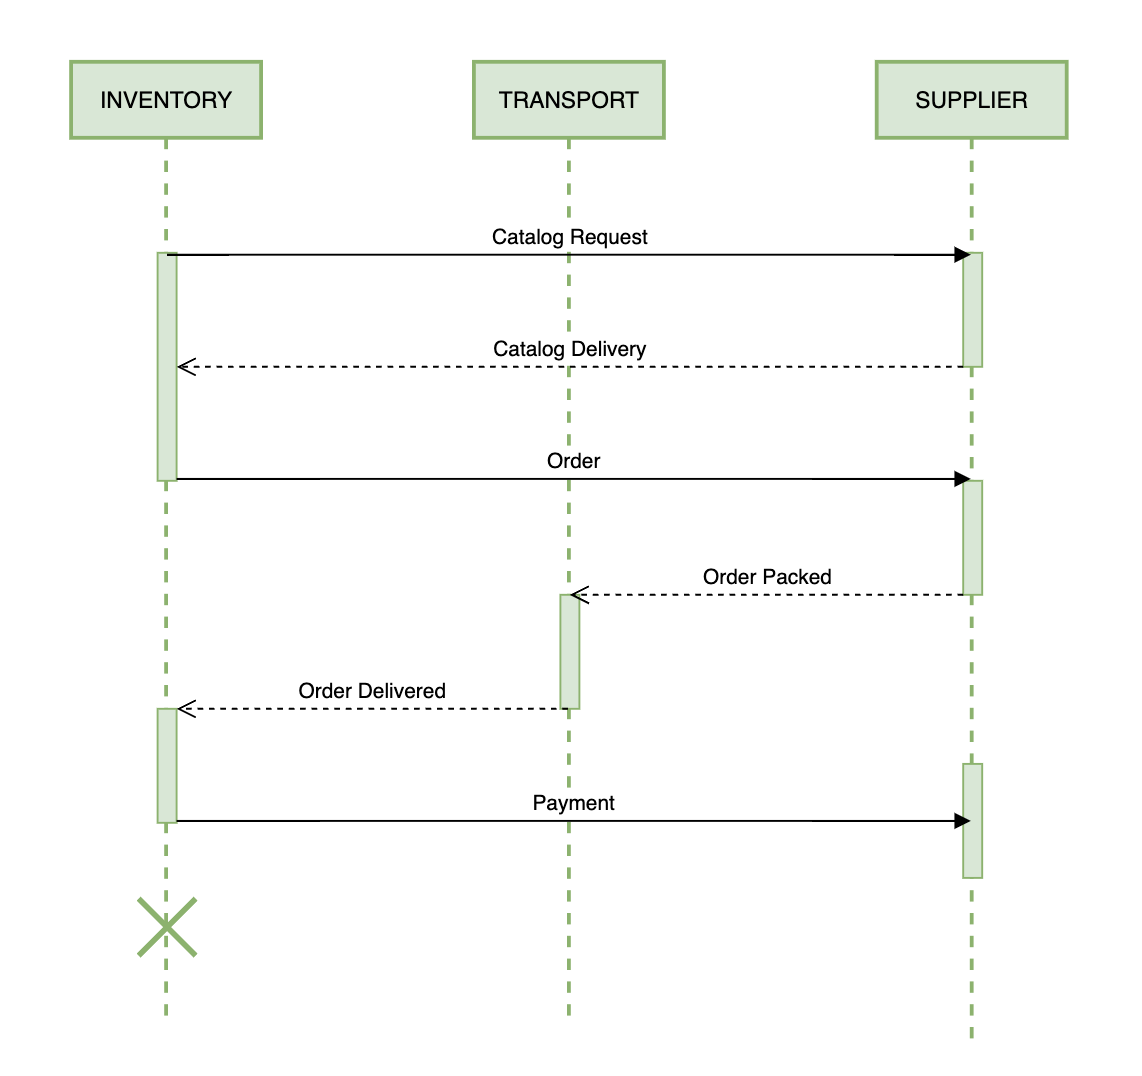
\includegraphics[scale = 0.5]{Sequence Diagram 2.png}
\end{center}
\section{\textbf{Conclusion}}
Hence, I learned to draw Sequence Diagram.
\section{\textbf{Platform Used:}}
\begin{itemize}
	\item \textbf{Operating System:} Mac OS 64-bit
	\item \textbf{Input:} Problem Statement Scenario
	\item \textbf{Output:} Sequence Diagram
\end{itemize}
\section{\textbf{FAQ's}}
\subsection{\textit{Give the significance of dynamic diagrams in UML.}}
\textbf{Ans.} Dynamic diagrams in the Unified Modeling Language (UML) are used to describe the behavior of a system over time. They are particularly useful for modeling complex interactions between objects and for specifying the flow of control between different components in a system.\\

There are several types of dynamic diagrams in UML, including sequence diagrams, collaboration diagrams, activity diagrams, state machine diagrams, and timing diagrams. Each of these diagrams has its own specific purpose and is used to model different aspects of system behavior.\\

The significance of dynamic diagrams in UML is that they allow developers to visualize and analyze the behavior of a system in a clear and structured way. By modeling the interactions between objects and the flow of control between components, dynamic diagrams can help developers identify potential problems and optimize system performance.\\

In addition, dynamic diagrams can be used to document and communicate the behavior of a system to stakeholders, such as project managers, customers, and other members of a development team. This can help ensure that everyone involved in the project has a clear understanding of how the system is intended to function and can facilitate effective collaboration and communication.

\subsection{\textit{Explain any 2 Terminologies Used in Sequence Diagrams}}
\textbf{Ans.} Sequence diagrams are a type of dynamic diagram in UML that show the interactions between objects in a system over time. They are used to model the behavior of a system in terms of messages passed between objects and the order in which those messages are sent and received.\\

Here are two terminologies used in sequence diagrams:
\begin{enumerate}
	\item \textbf{Lifeline:} In a sequence diagram, a lifeline represents an object in the system that participates in a particular sequence of interactions. A lifeline is depicted as a vertical line that extends downwards from the object name, and it typically shows the lifetime of an object during the sequence of interactions. Messages are exchanged between lifelines to show the order in which interactions occur.
	\item \textbf{Message:} A message is an action that is sent from one object to another in a sequence diagram. Messages can be synchronous, asynchronous, or a reply. A synchronous message is one in which the sender object waits for a response from the receiver object before continuing. An asynchronous message is one in which the sender object does not wait for a response from the receiver object and continues processing. A reply message is a response to a synchronous message and indicates that the receiver object has completed processing and sent a response back to the sender object.

\end{enumerate}
Understanding these two terminologies is important for creating accurate and meaningful sequence diagrams. By using lifelines and messages, developers can model the behavior of a system in a way that is easy to understand and communicate to others involved in the project.
\subsection{\textit{Explain the message passing in Sequence Diagrams}}
\textbf{Ans.} In a sequence diagram, message passing refers to the exchange of messages between objects in a system. Messages are used to represent the communication that occurs between objects as they collaborate to achieve a particular task.\\

When modeling message passing in a sequence diagram, there are several important aspects to consider:
\begin{itemize}
	\item \textbf{Message type:} There are three types of messages in a sequence diagram - synchronous, asynchronous, and reply messages. A synchronous message is one in which the sender object waits for a response from the receiver object before continuing. An asynchronous message is one in which the sender object does not wait for a response from the receiver object and continues processing. A reply message is a response to a synchronous message and indicates that the receiver object has completed processing and sent a response back to the sender object.
	\item \textbf{Message name:} The name of a message in a sequence diagram should describe the action being taken or the information being passed between objects. This can help make the diagram more clear and understandable.
	\item \textbf{Message parameters:} Messages in a sequence diagram can have parameters, which are used to pass data or other information between objects. Parameters can be simple values, such as integers or strings, or more complex data structures, such as arrays or objects.
	\item \textbf{Message ordering:} In a sequence diagram, messages are shown in the order in which they occur. The ordering of messages is important for understanding the flow of control and the behavior of the system.

\end{itemize}
By modeling message passing in a sequence diagram, developers can gain a better understanding of how objects in a system collaborate to achieve a particular task. This can help identify potential problems or bottlenecks in the system and optimize its performance.
\end{document}